\documentclass[xcolor=dvipsnames,slidestop, mathserif]{beamer}
\usepackage{amsmath}
\usepackage[utf8]{inputenc}
\usepackage[T1]{fontenc}

\usepackage{graphicx}
\usepackage[ruled,linesnumbered,noend,nofillcomment,scleft]{algorithm2e}
\usepackage{setspace}
\usepackage{listings}
\usepackage{hyperref}
\usepackage{subfigure}
\usepackage{booktabs,longtable,tabularx,ltxtable,subfigure,ragged2e}%

\useoutertheme{infolines} 
\usepackage{beamerthemeshadow}

\usepackage{color, colortbl}
\usepackage[dvipsnames]{xcolor}

\usepackage{dirtree}
\usepackage{cleveref}% it must be the last package

\makeatletter
\definecolor{Gray}{gray}{0.7}

\newcommand\YAMLcolonstyle{\color{red}\mdseries}
\newcommand\YAMLkeystyle{\color{black}\bf\bfseries\ttfamily\scriptsize}
\newcommand\YAMLvaluestyle{\color{blue}\mdseries}

\newcommand\language@yaml{yaml}
\expandafter\expandafter\expandafter\lstdefinelanguage
\expandafter{\language@yaml}
{
  keywords={true,false,null,y,n},
  keywordstyle=\color{darkgray}\bfseries,
  basicstyle=\YAMLkeystyle,                                 % assuming a key comes first
  showspaces=false,
  showstringspaces=false,
  sensitive=false,
  comment=[l]{\#},
  morecomment=[s]{/*}{*/},
  commentstyle=\color{purple}\ttfamily,
  stringstyle=\YAMLvaluestyle\ttfamily,
  moredelim=[l][\color{orange}]{\&},
  moredelim=[l][\color{magenta}]{*},
  moredelim=**[il][\YAMLcolonstyle{:}\YAMLvaluestyle]{:},   % switch to value style at :
  morestring=[b]',
  morestring=[b]",
  literate =    {---}{{\ProcessThreeDashes}}3
                {>}{{\textcolor{red}\textgreater}}1     
                {|}{{\textcolor{red}\textbar}}1 
                {\ -\ }{{\mdseries\ -\ }}3,
}

% switch to key style at EOL
\lst@AddToHook{EveryLine}{\ifx\lst@language\language@yaml\YAMLkeystyle\fi}
\makeatother

\newcommand\ProcessThreeDashes{\llap{\color{cyan}\mdseries-{-}-}}

\lstset{
   backgroundcolor=\color{white},   % choose the background color;
   basicstyle=\footnotesize,        % the size of the fonts that are used for the code;
   captionpos=b,                    % sets the caption-position to bottom;
   breaklines=true,                 % sets automatic line breaking;
   numberstyle=\tiny\color{gray},   % the style that is used for the line-numbers;
   %numbers=right,                  % sets the line number position;
   numbersep=1pt,                   % sets the distance between the line number and the text;
   xleftmargin=.1in,                % sets the left margin;
   xrightmargin=.1in,               % sets the right margin;
   commentstyle=\color{darkgreen},  % choose the comment color;
}

%%%%%%%%%%%%%%%%%%%%%%%%%%%%%%%%%%%%%%%%%%%%%%%%%%%%%%%%%%%%%%%%%%

\newcommand{\mcbf}[2]{\multicolumn{#1}{c}{\textbf{#2}}}

\graphicspath
{
    {figures/}%
}

%%%%%%%%%%%%%%%%%%%%%%%%%%%%%%%%%%%%%%%%%%%%%%%%%%%%%%%%%%%%%%%%%%
\input{beamer-fix}
%http://comments.gmane.org/gmane.editors.lyx.general/72441
\setbeamercovered{transparent=25}
\setbeamertemplate{caption}[numbered]

\setbeamertemplate{navigation symbols}{}%remove navigation symbols The simplest way is: \beamertemplatenavigationsymbolsempty
\setbeamertemplate{note page}[infolines]

%\setbeameroption{show only notes}
%\setbeameroption{show notes}
%http://www.phillme.de/cms/node/14
%\setbeameroption{show notes on second screen} %more details and example in http://tug.org/pracjourn/2010-1/dohmen/


\title[\hspace{.4in}\insertframenumber/\inserttotalframenumber]{Ansible Hands-On}
\author{DevOps Bras\'ilia}

\begin{document}

\singlespacing 
\begin{frame}[plain]
  \titlepage
\end{frame}

% \section*{Outline}
% \begin{frame}[plain]{Outline}
%   \tableofcontents[hideallsubsections]
% \end{frame}

% \AtBeginSection[]
% {
% \begin{frame}[plain]
%  \frametitle{Outline}
%  \footnotesize{\tableofcontents[currentsection,hideothersubsections]}
% \end{frame}
% }

\begin{frame}{Deploy an application manually is usually time-consuming}
	\begin{itemize}
	   \item Most of the applications rely on different services to work correctly
     \item These services usually run on a distributed set of computing resources and communicate using various networking protocols
	   \item Wire up these services by hand is time-consuming, error-prone, and it makes difficult to implement continuous delivery, for instance.
	   \item Therefore, one way to deal with this problem is to use configuration management tools like Ansible, Chef, Puppet, Salt, among others.
	\end{itemize}	
\end{frame}

\begin{frame}{What do we mean by configuration management?}
  \begin{itemize}
     \item Writing the states for the servers, and then, using a tool to enforce that the servers are in the required state:
       \begin{enumerate}
          \item the right packages are installed
	        \item the configuration files contain the expected values and the correct permissions
	        \item the right services are running
	        \item $\cdots$
       \end{enumerate} 
  \end{itemize}
\end{frame}

\begin{frame}{What can we expect from configuration management tools?}
   \begin{itemize}
      \item they can help us on implementing continuous delivery, i.e., on implementing the blue-green deployment approach\footnotemark.
      \item on dealing with deployment orchestration. In other words, when there are multiple servers involved and the tasks must happen in a specific order. For instance, a database must be set up before bringing up the application servers.
      \item they can provision new servers. In the context of IaaS cloud, this means to spinning up new virtual machine instance.
      \item they help on guarantee the~\textit{idempotence} property.
   \end{itemize}
   \footnotetext[1]{martinfowler.com/bliki/BlueGreenDeployment.html}
\end{frame}	

\begin{frame}{And Ansible, what is it Good For?}
  \begin{itemize}
     \item For describing the state of the servers through its DSL
     \item For doing deployment as well as configuration management
     \item For performing actions on multiple servers with a simple state model
     \item For control the order that the actions must happen in
     \item For talking to the public clouds API (e.g., AWS EC2, Google Compute Engine, Azure), as well as any cloud that supports the OpenStack API
  \end{itemize}
\end{frame}

\begin{frame}{How Ansible works}
\vspace{-0.5cm}
  \begin{figure}
     \centering
     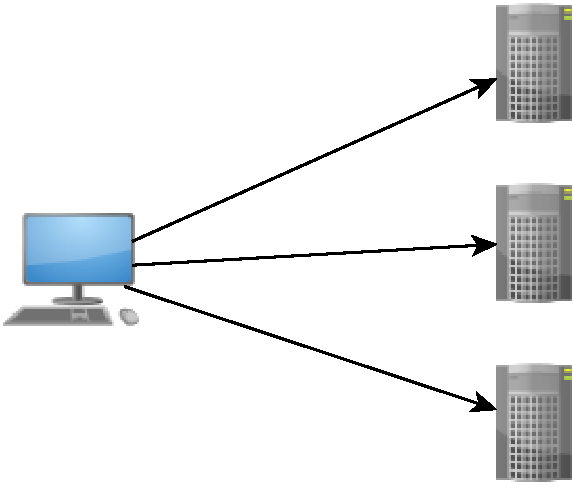
\includegraphics[width=.4\columnwidth]{ansible-working-example}
     \caption{Using Ansible to perform actions on three remote servers}
  \end{figure}

  \begin{enumerate}
    \item it makes an SSH connection for each server
    \item it executes the first task on all the three nodes simultaneously:
       \begin{enumerate}
          \item generate a Python script that represents the task
          \item copy the script to the servers
          \item execute the script on the nodes
          \item wait for the script to complete on all the hosts
       \end{enumerate}
  \end{enumerate}
\end{frame}

\begin{frame}{What are good Ansible's characteristics?}
   \begin{itemize}
     \item Easy-to-read syntax: its script (i.e., playbook) is built on top of the YAML format
     \item Nothing to install on the remote servers
     \item Push-based: it is the developer who controls when the changes happens to the servers
     \item Built-in modules: there are many modules to perform the tasks. Modules are idempotent
     \item A very thin layer of abstraction: we don't need to learn a new package manager
     \item It has a low learning curve
   \end{itemize}
\end{frame}

\begin{frame}{Setup Environment}
\vspace{-0.6cm}
  \begin{figure}
     \centering
     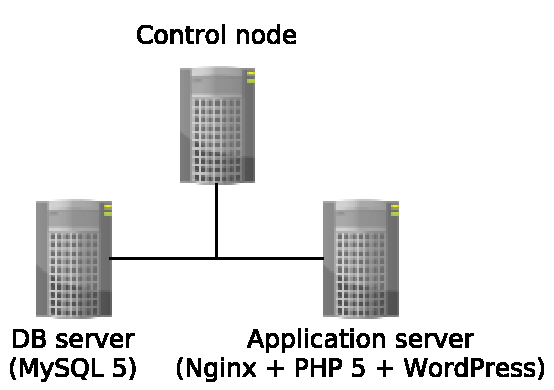
\includegraphics{environment-configuration}
     \caption{We will use Ansible to deploy WordPress with services running on two different nodes}
  \end{figure}
\end{frame}

\begin{frame}[fragile]{Starting with Ansible}
  \begin{enumerate}
    \item Provision the virtual machines and connect to the control node
    \begin{lstlisting}[language=Bash]
       vagrant up
       vagrant ssh
    \end{lstlisting}
    \item Create an inventory file to inform Ansible what are the remote servers, as well as how to connect to them.
    \item Write the configuration scripts
    \item Push the configuration scripts to the remote nodes
  \end{enumerate}
\end{frame}

\begin{frame}[fragile]{Ansible's inventory file}
\vspace{-0.4cm}
\lstinputlisting[
      breaklines=true,
      escapechar=@,
      frame=tb,
      language=yaml,
      basicstyle=\ttfamily\scriptsize,
      showspaces=false,
      showstringspaces=false,
      caption={Example of an inventory file (i.e., ansible.cfg)},
]{../playbooks/ansible.cfg}

\lstinputlisting[
      language=yaml,
      basicstyle=\ttfamily\scriptsize,
      showspaces=false,
      showstringspaces=false,
      frame=tb,
      caption={Example of a host file},
]{../playbooks/hosts}

\begin{itemize}
  \item By default, Ansible looks for an inventory file (\emph{ansible.cfg}) in:
    \begin{enumerate}
      \item \emph{ANSIBLE$\_$CONFIG$\_$ENVIRONMENT} variable
      \item \textit{./ansible.cfg}
      \item \textit{\$HOME/.ansible.cfg}
      \item /etc/ansible/ansible.cfg
    \end{enumerate}
\end{itemize}
\end{frame}

\begin{frame}[fragile]{Ansible's hello world}
  \begin{lstlisting}[language=yaml] 
     ansible all -i hosts -m ping 
  \end{lstlisting}
  or only
  \begin{lstlisting}[language=yaml] 
     ansible all -m ping 
  \end{lstlisting}
    where,
     \begin{itemize}
        \item \textbf{all} is the target hosts
        \item \textbf{hosts} is the host lists
        \item \textbf{ping} is the module (i.e., action) to execute
     \end{itemize}
\end{frame}

\begin{frame}{Default structure of an Ansible's project}
\dirtree%
{%
.1 /\underline{playbooks}.
.2 \underline{files}.
.3 static file$_1$.
.3 static file$_2$.
.3 $\vdots$.
.3 static file$_n$.
.2 \underline{templates}.
.3 template file$_1$.j2.
.3 template file$_2$.j2.
.3 $\vdots$.
.3 template file$_n$.
.2 ansible.cfg
.2 hosts
.2 playbook$_1$.yml.
.2 playbook$_2$.yml.
.2 $\vdots$.
.2 playbook$_n$.yml.
}%
\end{frame}

\begin{frame}{Ansible's script: Playbook}
  \begin{block}{Playbook}
  A playbook is the term that Ansible uses for describe a configuration management script. In practice, it is a list of plays.
  \end{block}

  \begin{figure}
     \centering
     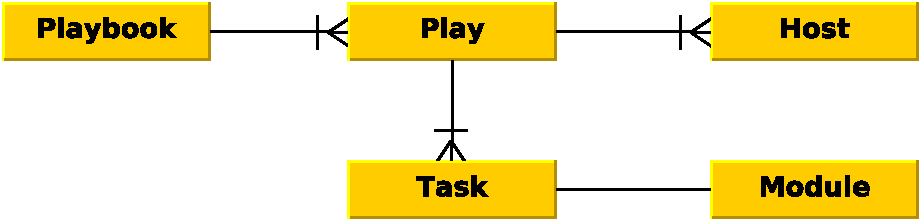
\includegraphics[width=.8\columnwidth]{playbook}
     \caption{Representing Ansible's playbook elements}
  \end{figure}
\end{frame}

\begin{frame}[fragile]{Ansible's script: Playbook}
\vspace{-0.5cm}
  \begin{figure}
     \centering
     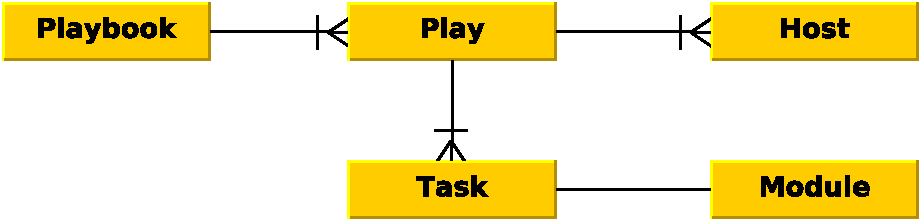
\includegraphics[width=.4\columnwidth]{playbook}
     \caption{Representing Ansible's playbook elements}
  \end{figure}
\vspace{-0.5cm}
  \begin{block}{What is a play?}
     A play associates an unordered set of hosts with an ordered list of tasks. A play must have:
     \begin{itemize}
        \item a set of hosts to configure
        \item a lits of tasks to be executed in the hosts
     \end{itemize}
    Additionally, a play may also have:
    \begin{itemize}
        \item a \textbf{name}: a comment that describes what the play is about
        \item \textbf{become} and \textbf{become$\_$method}: tell Ansible if the tasks must be executed as root 
        \item \textbf{vars} a list of variables and values to be used in the play.
     \end{itemize}
  \end{block}
\end{frame}

\begin{frame}[fragile]{Ansible's script: Playbook}
\vspace{-0.5cm}
  \begin{figure}
     \centering
     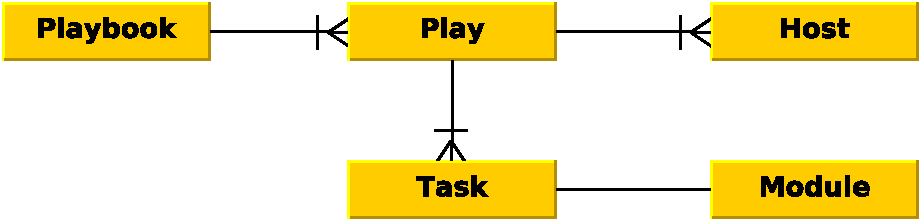
\includegraphics[width=.4\columnwidth]{playbook}
     \caption{Representing Ansible's playbook elements}
  \end{figure}
\vspace{-0.5cm}
  \begin{block}{What is a task?}
     A task is the action to execute on the host. Every task must contain:
     \begin{itemize}
        \item a \textbf{key} with the name of a module
        \item a \textbf{value} with the arguments of the module.
     \end{itemize}
     \begin{lstlisting}[language=yaml,basicstyle=\ttfamily\scriptsize,
showspaces=false,showstringspaces=false,frame=tb]
tasks:
  - name: install ngix
    apt: name=nginx update_cache=yes cache_valid_time=3600
     \end{lstlisting}
  \end{block}
\end{frame}

\begin{frame}[fragile]{Playbooks support the usage of variables}
\begin{itemize}
  \item Variables can be used in tasks and in templates files.
  \item A variable's value can be: string, boolean, lists, and dictionaries.
  \item To reference a variable, we use the brace $\{\{$ var$\_$name $\}\}$ notation.
  \item Ansible uses Jinja2\footnotemark template engine to evaluate variables in playbooks and in template files.
\end{itemize}
\begin{lstlisting}[language=yaml,frame=tb,caption={Example of defining and referencing a variable}]
vars:
    cert_file: /etc/nginx/ssl/nginx.crt
tasks:
  - name: copy the TLS certificate
    copy: src=nginx.crt dest={{ cert_file }}
\end{lstlisting}

\begin{itemize}
  \item Ansible also allows us to put the variables into one or more files, and reference them through the \textbf{vars$\_$files} section.
\end{itemize}
\begin{lstlisting}[language=yaml,frame=tb,caption={Example of defining the variables in separate files}]
vars_files:
    - nginx.yml
tasks:
  - name: copy the TLS certificate
    copy: src=nginx.crt dest={{ cert_file }}
\end{lstlisting}
\footnotetext[2]{jinja.pocoo.org/docs/dev}
\end{frame}

\begin{frame}[fragile]{Playbooks support the usage of variables}
  \begin{itemize}
    \item Variables can be defined at runtime, using the \textbf{register} clause when executing a task.
    \item In this case, the type of the variable is always a dictionary, and its keys depend of the modules.
    \item the debug task can be used to know the value of a variable.
  \end{itemize}
\begin{lstlisting}[language=yaml, frame=tb,escapechar=@]
tasks:
  - name: register the output of whoami command
    command: whoami
    @\textbf{register}@: login_user
  - debug: msg="Logged as user: {{ login_user.stdout }}"
\end{lstlisting}
\end{frame}

\begin{frame}[fragile]{Built-in variables}
\vspace{-0.8cm}
\begin{table}
\scriptsize
{
  \begin{tabular}{rl}
    \hline \textbf{Name} & \textbf{Description} \\ \hline
    \textbf{hostvars} & a dictionary whose keys are Ansible hostnames and values are \\
    & dictionaries that map variables names to values. \\
    \textbf{inventory\_hostname} & name of the current host as defined in the inventory file.\\
    \textbf{group\_names} & a list of all groups that the current node is member of \\
    \textbf{groups} & a dictionary whose keys are Ansible group names and values are list of \\
    & hostnames that are member of the group. \\
    \textbf{play\_hosts} & a list of the hostnames of the current play. \\
    \textbf{ansible\_version} & a dictionary with the Ansible's version. \\
    \hline
  \end{tabular} 
}
\end{table}
\scriptsize
\vspace{-0.3cm}
\begin{itemize}
  \item Ansible can also provide information about the node, such as IP addresses, memory size, disk, operating system, etc.
  % \item for this, we need to demand Ansible to collect the data, defining \textbf{gather\_facts: yes} in a playbook.
  \end{itemize}

\begin{lstlisting}[language=yaml,frame=tb]
---
- name: collect the name of the user and the facts about the node
  hosts: webservers
  gather_facts: yes
  tasks:
    - name: register the output of whoami command
      command: whoami
      register: login_user
    - debug: msg="Logged as user {{ login_user.stdout }} and my IP address is {{ hostvars[groups['webservers'][0]]['ansible_eth1']['ipv4']['address'] }}"
\end{lstlisting}

\end{frame}

% - name: install MySQL server
%       apt: name={{ item }} update_cache=yes cache_valid_time=3600 state=present
%       with_items:
%         - mysql-server
%         - python-mysqldb

\begin{frame}[fragile]{Using Handler to notify a new state}
\begin{itemize}
  \item A handler is similar to a tasks, but it only runs if it has be notified by a task.
  \item A task only fires a notification only if the node's state has changed.
  \item Handlers only run after all of the tasks have finished, and they only run once, even if they are notified multiple times.
  \item Handlers always run in the order that they appear in the play,  and not in the notification order.
\end{itemize}

\begin{lstlisting}[language=yaml,frame=tb]
  tasks:
    - name: copy the TLS key
      copy: src=files/nginx.key dest={{ key_file }} owner=root mode=0600
      notify: restart nginx
  handlers:
    - name: restart nginx
      service: name=nginx state=restarted
\end{lstlisting}

\end{frame}


% \begin{frame}{}
% {
% \usebackgroundtemplate{\includegraphics[width=\paperwidth,height=\paperheight]{thatsallfolks}}%width=\paperwidth
% \begin{frame}[plain]
%   % \vspace{0.8cm}
%   % \begin{block}{}
%   %    \LARGE \begin{center}Thank you!\end{center}
%   % \end{block}
  
%   % \vspace{0.8cm}
%   % \begin{block}{}
%   %    \LARGE \begin{center}Questions ?\end{center}
%   % \end{block}  
% \end{frame}
% }

\end{document}
